\documentclass[border=5pt]{standalone}
\usepackage{amsmath,amssymb}
\usepackage{xcolor}
\usepackage{tikz}
\usetikzlibrary{positioning,arrows.meta,fit,backgrounds,calc,shapes.geometric}
\definecolor{cset}{RGB}{31,119,180}
\definecolor{cfield}{RGB}{44,160,44}
\definecolor{cop}{RGB}{214,39,40}
\definecolor{cgray}{RGB}{120,120,120}
\begin{document}
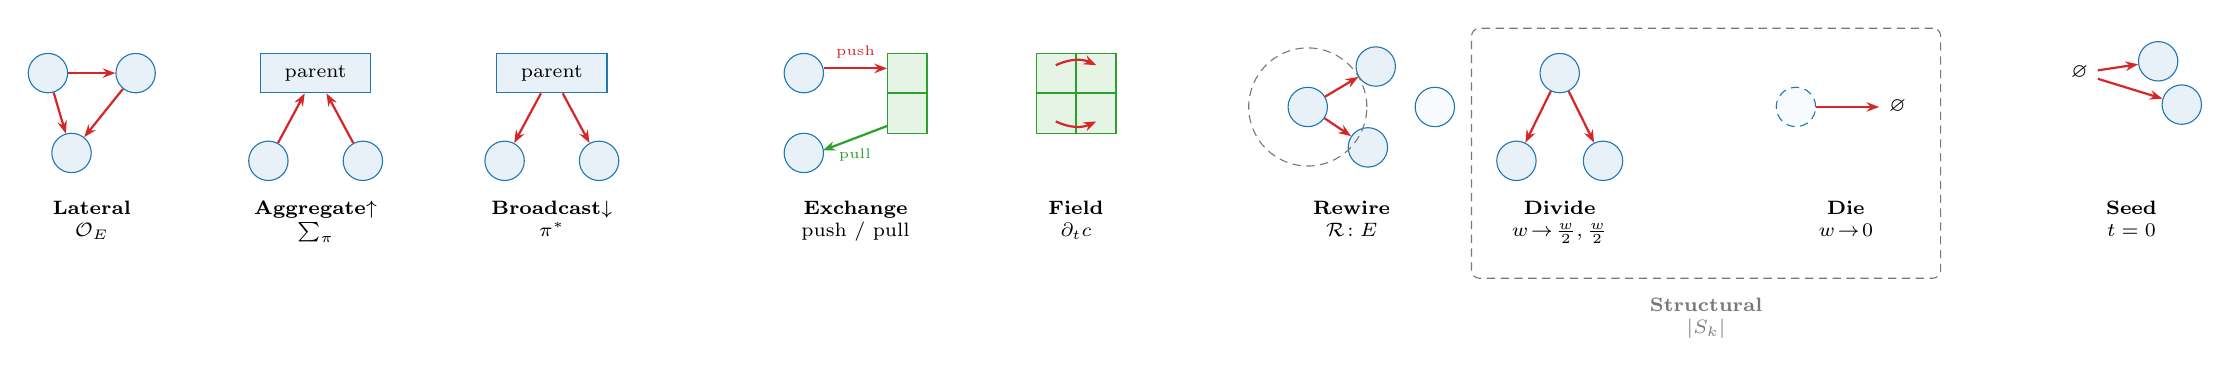
\begin{tikzpicture}[
  font=\scriptsize,
  n/.style={circle,draw=cset,fill=cset!10,minimum size=5mm,inner sep=0},
  p/.style={rectangle,draw=cset,fill=cset!10,minimum width=14mm,minimum height=5mm},
  g/.style={rectangle,draw=cfield,fill=cfield!12,minimum width=5mm,minimum height=5mm},
  a/.style={-{Stealth[length=1.6mm]},cop,thick},
]
\begin{scope}[local bounding box=L]
  \node[n] (a1){}; \node[n,right=6mm of a1](a2){}; \node[n,below=5mm of a1,xshift=3mm](a3){};
  \draw[a] (a1)--(a2); \draw[a] (a1)--(a3); \draw[a] (a2)--(a3);
\end{scope}
\node[anchor=north,align=center] at (L |- 0,-15mm){\textbf{Lateral}\\$\mathcal{O}_E$};
\begin{scope}[shift={(34mm,0)},local bounding box=A]
  \node[p] (par){parent};
  \node[n,below=6mm of par,xshift=-6mm](c1){}; \node[n,below=6mm of par,xshift=6mm](c2){};
  \draw[a] (c1)--(par); \draw[a] (c2)--(par);
\end{scope}
\node[anchor=north,align=center] at (A |- 0,-15mm){\textbf{Aggregate}$\uparrow$\\$\sum_\pi$};
\begin{scope}[shift={(64mm,0)},local bounding box=B]
  \node[p] (par2){parent};
  \node[n,below=6mm of par2,xshift=-6mm](d1){}; \node[n,below=6mm of par2,xshift=6mm](d2){};
  \draw[a] (par2)--(d1); \draw[a] (par2)--(d2);
\end{scope}
\node[anchor=north,align=center] at (B |- 0,-15mm){\textbf{Broadcast}$\downarrow$\\$\pi^*$};
\begin{scope}[shift={(96mm,0)},local bounding box=E]
  \node[n] (o1){}; \node[n,below=5mm of o1](o2){};
  \node[g,right=8mm of o1](g1){}; \node[g,below=0mm of g1](g2){};
  \draw[a,transform canvas={yshift=0.6mm}] (o1)-- node[above,font=\tiny]{push}(g1);
  \draw[a,cfield,transform canvas={yshift=-0.6mm}] (g2)-- node[below,font=\tiny]{pull}(o2);
\end{scope}
\node[anchor=north,align=center] at (E |- 0,-15mm){\textbf{Exchange}\\push / pull};
\begin{scope}[shift={(128mm,0)},local bounding box=FD]
  \node[g] (f1){}; \node[g,right=0mm of f1](f2){}; \node[g,below=0mm of f1](f3){};
  \node[g,below=0mm of f2](f4){};
  \draw[a] ($(f1.center)+(0,1mm)$) to[bend left=25] ($(f2.center)+(0,1mm)$);
  \draw[a] ($(f3.center)-(0,1mm)$) to[bend right=25] ($(f4.center)-(0,1mm)$);
\end{scope}
\node[anchor=north,align=center] at (FD |- 0,-15mm){\textbf{Field}\\$\partial_t c$};
% --- structure operators: Rewire (edges E), Divide / Die (node set |S|) ---
\begin{scope}[shift={(160mm,-4.3mm)},local bounding box=RW]
  \node[n] (rc){};
  \node[n,above right=1.5mm and 5mm of rc](rn1){};
  \node[n,below right=1.5mm and 4mm of rc](rn2){};
  \node[n,right=11mm of rc,fill=cset!3](rn3){};
  \draw[densely dashed,cgray] (rc) circle (7.5mm);
  \draw[a] (rc)--(rn1); \draw[a] (rc)--(rn2);
\end{scope}
\node[anchor=north,align=center] at (RW |- 0,-15mm){\textbf{Rewire}\\$\mathcal{R}\!:E$};
\begin{scope}[shift={(192mm,0)},local bounding box=DV]
  \node[n] (m){};
  \node[n,below=6mm of m,xshift=-5.5mm](g3){}; \node[n,below=6mm of m,xshift=5.5mm](g4){};
  \draw[a] (m)--(g3); \draw[a] (m)--(g4);
\end{scope}
\node[anchor=north,align=center] (DVL) at (DV |- 0,-15mm){\textbf{Divide}\\$w\!\to\!\tfrac{w}{2},\tfrac{w}{2}$};
\begin{scope}[shift={(222mm,-4.3mm)},local bounding box=DE]
  \node[n,densely dashed,fill=cset!3] (z){};
  \node[right=8mm of z] (nul) {$\varnothing$};
  \draw[a] (z)--(nul);
\end{scope}
\node[anchor=north,align=center] (DEL) at (DE |- 0,-15mm){\textbf{Die}\\$w\!\to\!0$};
% ONE KIND, TWO OPERATORS. `structural` is what the registry calls the kind that changes the node
% set; Divide and Die are its two members, so they are drawn inside it rather than beside it.
\begin{scope}[on background layer]
  \node[draw=cgray,densely dashed,rounded corners=1mm,inner sep=3.2mm,
        fit=(DV)(DE)(DVL)(DEL)] (STR) {};
\end{scope}
\node[anchor=north,align=center,cgray] at ($(STR.south)-(0,1.2mm)$){\textbf{Structural}\\$|S_k|$};
\begin{scope}[shift={(258mm,0)},local bounding box=SD]
  \node (sv) at (0,0) {$\varnothing$};
  \node[n] (s1) at (10mm,1.5mm){}; \node[n] (s2) at (13mm,-4mm){};
  \draw[a] (sv)--(s1); \draw[a] (sv)--(s2);
\end{scope}
\node[anchor=north,align=center] at (SD |- 0,-15mm){\textbf{Seed}\\$t=0$};
\end{tikzpicture}
\end{document}
